\documentclass[11pt, fleqn]{article}

\usepackage{amsmath}
\usepackage{amsfonts}
\usepackage{amsthm}
\usepackage[margin=1in]{geometry} % To set the margin widths
\usepackage{graphicx}
%\usepackage{hyperref}
\usepackage{listings}
\usepackage{multirow}
\usepackage{tabularx}
\usepackage{varioref}
\usepackage{cleveref}  % this redefines vref to use cleverref
\usepackage{siunitx}
%\usepackage{subcaption}
\usepackage{subfig}
\usepackage{titlesec}
\usepackage{bm}

\crefname{equation}{equation}{equations}
\crefname{figure}{figure}{figures}

\sisetup{output-exponent-marker=\textsc{e}}

\titleformat{\section}[block]{\bfseries}{\thesection}{1em}{}


\setlength{\parskip}{12pt} % Sets a blank line in between paragraphs
\setlength\parindent{0pt} % Sets the indent for each paragraph to zero

\begin{document}

\title{Big Data: Homework 4}
\author{Will Clark \& Matthew DeLio \\ 41201-01}
\date{\today}
\maketitle

\section{Node Connectivity Transformation}

Node connectivity (which we are calling \texttt{degree}) is measured by the number of edges for each node in a network. In this context, \texttt{degree} tells us the number of relationships that a household in our population has. We observe in Figure~\ref{fig:degrees} that \texttt{degree} is distributed logarithmically.

\begin{figure}[!htb]
  \centering
  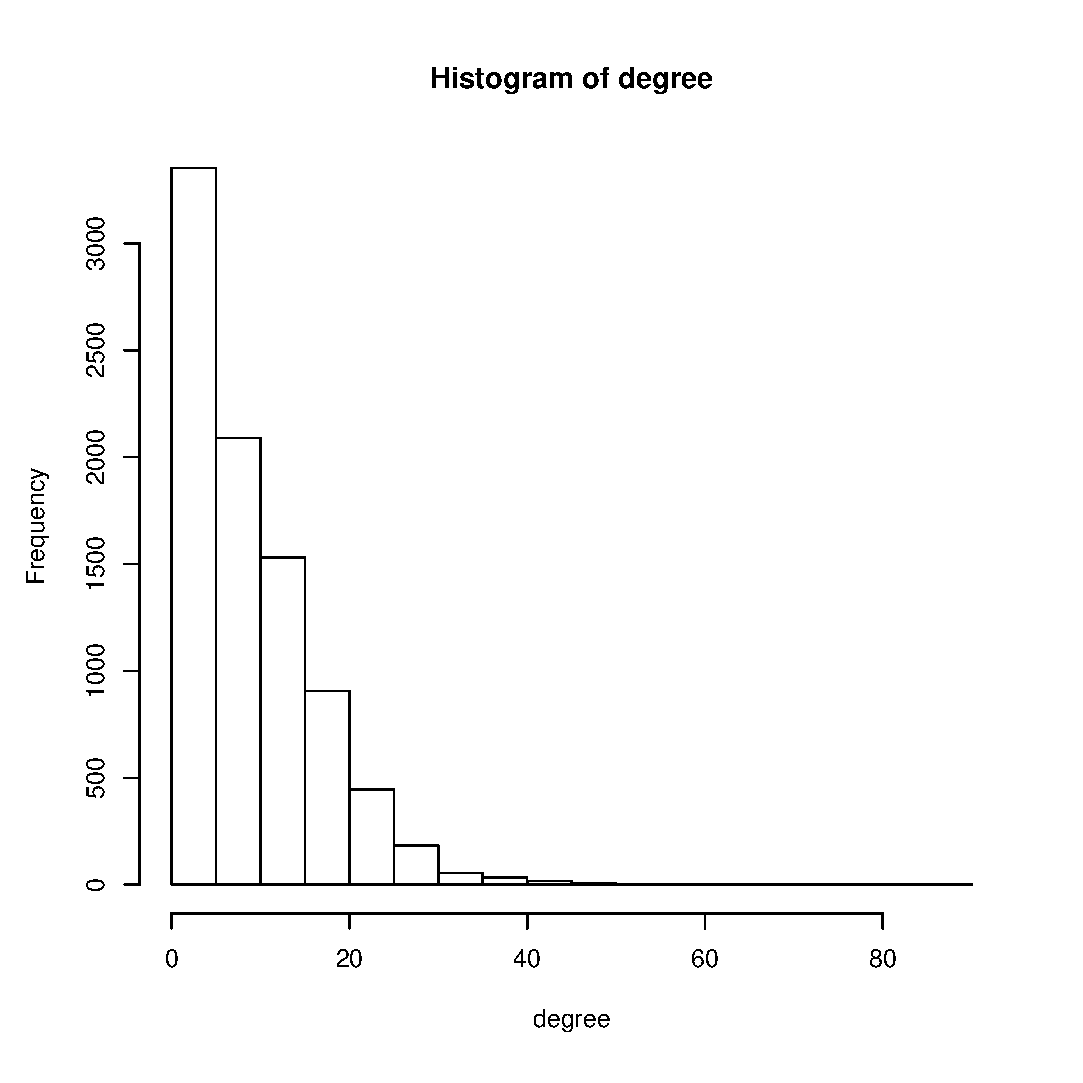
\includegraphics[scale=.5]{degrees.eps}
  \caption{Distribution of \texttt{degree}}
  \label{fig:degrees}
\end{figure}

\section{Predicting Node Connectivity from Controls}
\label{sec:predict}

In this section, we build a model to predict a node's degree by using only our control variables. Our model is: 

\[ d = \beta_0 + \bm{X} \bm{\beta} + \varepsilon \]

where $d$ is a node's number of degrees, $\bm{X}$ is a vector of control variables including village, religion, type of roof on home, rooms and beds in home, a dummy variable for having electricity in home, whether a home is owned, and whether the person is a ``leader'' in the village. 

We estimate this model using a Gamma-Lasso regression. In Figure~\ref{fig:treat_aic} in the Appendix, we show the Gamma-Lasso path plots with five decision criteria marked: AIC, AICc, BIC, CV.Min, and CV.1se. The $\log(\lambda)$ selected by AICc and by CV.Min are reasonably close to each other (-4.60 and -4.46, respectively, shown in Table~\ref{tab:treat_ic} in the Appendix), which provides us with a confirmation that our model is estimated reasonably well.

We then use the model selected by AICc to predict degree (which we will call $\hat{d}$). We plot $d$ against $\hat{d}$ in Figure~\ref{fig:d_vs_dhat} and see that there is only a very rough correlation between the two ($\sigma_{d,\hat{d}}=0.34$)

\begin{figure}[!htb]
  \centering
  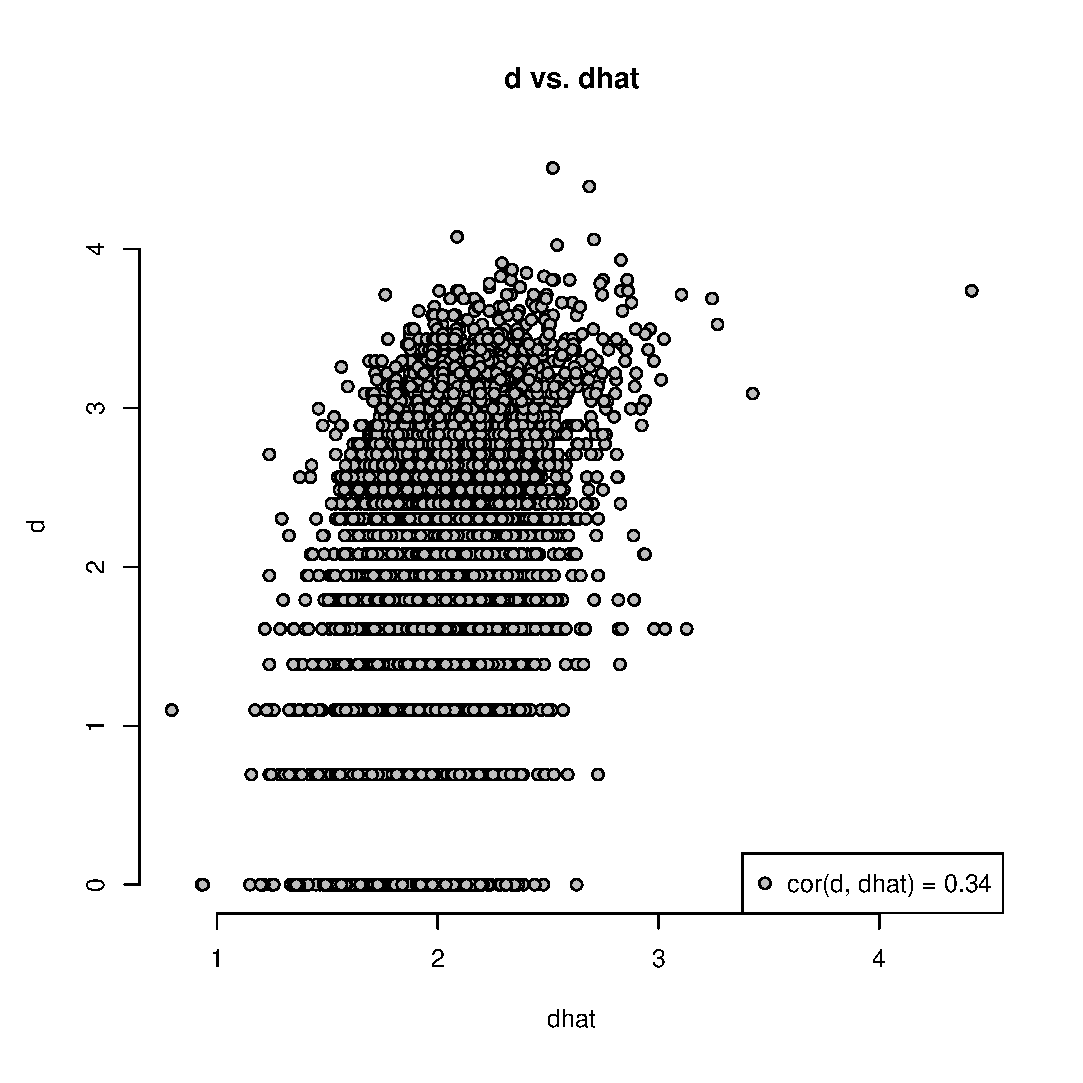
\includegraphics[scale=.5]{d_vs_dhat.eps}
  \caption{Degree and Predicted Degree}
  \label{fig:d_vs_dhat}
\end{figure}

This is a positive result. It tells us that most of the variation in degree, which will be our treatment variable in Section~\ref{sec:model}, is exogenous and cannot be explained by the control variables that we observe. We can therefore measure the effect of degree as a treatment on the propensity to take out a loan and be reasonably sure that we are not simply measuring variation in other observed control variables.

\section{Effect of Node Connectivity on Loan Propensity}
\label{sec:model}

\section{Naive Estimation of Loan Propensity}

\section{Bootstrapping Uncertainty}

\section{Experimental Design}

\section{Appendix}

\begin{figure}[!htb]
  \centering
  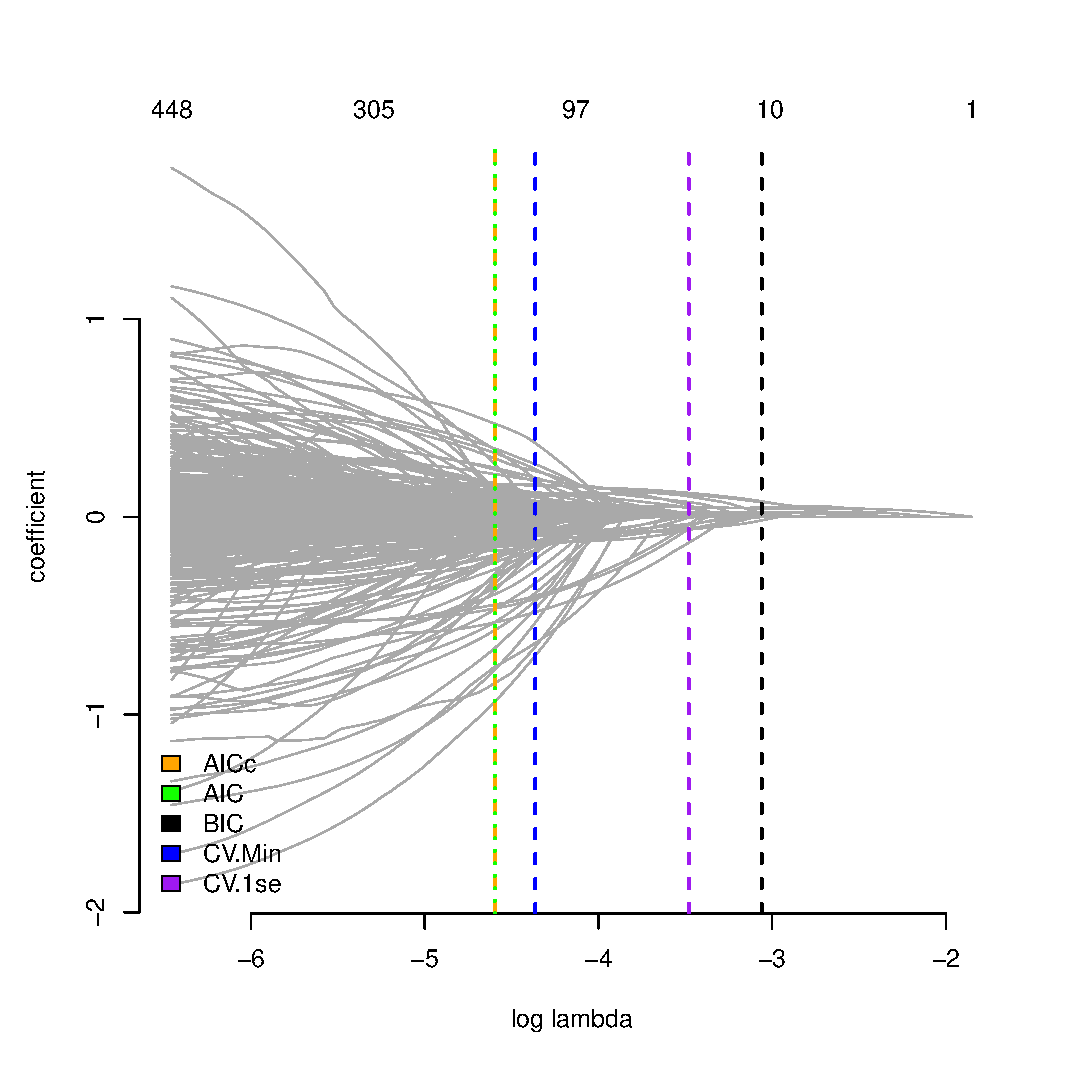
\includegraphics[scale=.5]{treat_aic.eps}
  \caption{Gamma-Lasso Regression for Degree on Controls}
  \label{fig:treat_aic}
\end{figure}

% latex table generated in R 3.0.2 by xtable 1.7-4 package
% Thu Apr 30 15:31:29 2015
\begin{table}[ht]
\centering
\begin{tabular}{rrr}
  \hline
 & $\log(\lambda)$ & Covariates Selected \\ 
  \hline
AICc & -4.60 & 185 \\ 
  AIC & -4.60 & 185 \\ 
  BIC & -3.06 &  10 \\ 
  CV.Min & -4.46 & 161 \\ 
  CV.1se & -3.53 &  37 \\ 
   \hline
\end{tabular}
\caption{Treatment IC Table} 
\label{tab:treat_ic}
\end{table}


\end{document}
